\documentclass[twoside]{book}

% Packages required by doxygen
\usepackage{fixltx2e}
\usepackage{calc}
\usepackage{doxygen}
\usepackage[export]{adjustbox} % also loads graphicx
\usepackage{graphicx}
\usepackage[utf8]{inputenc}
\usepackage{makeidx}
\usepackage{multicol}
\usepackage{multirow}
\PassOptionsToPackage{warn}{textcomp}
\usepackage{textcomp}
\usepackage[nointegrals]{wasysym}
\usepackage[table]{xcolor}

% Font selection
\usepackage[T1]{fontenc}
\usepackage[scaled=.90]{helvet}
\usepackage{courier}
\usepackage{amssymb}
\usepackage{sectsty}
\renewcommand{\familydefault}{\sfdefault}
\allsectionsfont{%
  \fontseries{bc}\selectfont%
  \color{darkgray}%
}
\renewcommand{\DoxyLabelFont}{%
  \fontseries{bc}\selectfont%
  \color{darkgray}%
}
\newcommand{\+}{\discretionary{\mbox{\scriptsize$\hookleftarrow$}}{}{}}

% Page & text layout
\usepackage{geometry}
\geometry{%
  a4paper,%
  top=2.5cm,%
  bottom=2.5cm,%
  left=2.5cm,%
  right=2.5cm%
}
\tolerance=750
\hfuzz=15pt
\hbadness=750
\setlength{\emergencystretch}{15pt}
\setlength{\parindent}{0cm}
\setlength{\parskip}{3ex plus 2ex minus 2ex}
\makeatletter
\renewcommand{\paragraph}{%
  \@startsection{paragraph}{4}{0ex}{-1.0ex}{1.0ex}{%
    \normalfont\normalsize\bfseries\SS@parafont%
  }%
}
\renewcommand{\subparagraph}{%
  \@startsection{subparagraph}{5}{0ex}{-1.0ex}{1.0ex}{%
    \normalfont\normalsize\bfseries\SS@subparafont%
  }%
}
\makeatother

% Headers & footers
\usepackage{fancyhdr}
\pagestyle{fancyplain}
\fancyhead[LE]{\fancyplain{}{\bfseries\thepage}}
\fancyhead[CE]{\fancyplain{}{}}
\fancyhead[RE]{\fancyplain{}{\bfseries\leftmark}}
\fancyhead[LO]{\fancyplain{}{\bfseries\rightmark}}
\fancyhead[CO]{\fancyplain{}{}}
\fancyhead[RO]{\fancyplain{}{\bfseries\thepage}}
\fancyfoot[LE]{\fancyplain{}{}}
\fancyfoot[CE]{\fancyplain{}{}}
\fancyfoot[RE]{\fancyplain{}{\bfseries\scriptsize Generated by Doxygen }}
\fancyfoot[LO]{\fancyplain{}{\bfseries\scriptsize Generated by Doxygen }}
\fancyfoot[CO]{\fancyplain{}{}}
\fancyfoot[RO]{\fancyplain{}{}}
\renewcommand{\footrulewidth}{0.4pt}
\renewcommand{\chaptermark}[1]{%
  \markboth{#1}{}%
}
\renewcommand{\sectionmark}[1]{%
  \markright{\thesection\ #1}%
}

% Indices & bibliography
\usepackage{natbib}
\usepackage[titles]{tocloft}
\setcounter{tocdepth}{3}
\setcounter{secnumdepth}{5}
\makeindex

% Hyperlinks (required, but should be loaded last)
\usepackage{ifpdf}
\ifpdf
  \usepackage[pdftex,pagebackref=true]{hyperref}
\else
  \usepackage[ps2pdf,pagebackref=true]{hyperref}
\fi
\hypersetup{%
  colorlinks=true,%
  linkcolor=blue,%
  citecolor=blue,%
  unicode%
}

% Custom commands
\newcommand{\clearemptydoublepage}{%
  \newpage{\pagestyle{empty}\cleardoublepage}%
}

\usepackage{caption}
\captionsetup{labelsep=space,justification=centering,font={bf},singlelinecheck=off,skip=4pt,position=top}

%===== C O N T E N T S =====

\begin{document}

% Titlepage & ToC
\hypersetup{pageanchor=false,
             bookmarksnumbered=true,
             pdfencoding=unicode
            }
\pagenumbering{alph}
\begin{titlepage}
\vspace*{7cm}
\begin{center}%
{\Large My Project }\\
\vspace*{1cm}
{\large Generated by Doxygen 1.8.13}\\
\end{center}
\end{titlepage}
\clearemptydoublepage
\pagenumbering{roman}
\tableofcontents
\clearemptydoublepage
\pagenumbering{arabic}
\hypersetup{pageanchor=true}

%--- Begin generated contents ---
\chapter{D\+A\+A1}
\label{md_README}
\Hypertarget{md_README}
Convex \hyperlink{classHull}{Hull} Algorithms

Build using make

T\+O\+DO\+:


\begin{DoxyEnumerate}
\item Add K\+PS
\item Check Small Testcases
\item Change some functions 
\end{DoxyEnumerate}
\chapter{Namespace Index}
\section{Namespace List}
Here is a list of all documented namespaces with brief descriptions\+:\begin{DoxyCompactList}
\item\contentsline{section}{\hyperlink{namespaceviz}{viz} }{\pageref{namespaceviz}}{}
\end{DoxyCompactList}

\chapter{Class Index}
\section{Class List}
Here are the classes, structs, unions and interfaces with brief descriptions\+:\begin{DoxyCompactList}
\item\contentsline{section}{\hyperlink{classHull}{Hull} }{\pageref{classHull}}{}
\item\contentsline{section}{\hyperlink{classPoint}{Point} }{\pageref{classPoint}}{}
\item\contentsline{section}{\hyperlink{classStack}{Stack} }{\pageref{classStack}}{}
\item\contentsline{section}{\hyperlink{classUtil}{Util} }{\pageref{classUtil}}{}
\end{DoxyCompactList}

\chapter{File Index}
\section{File List}
Here is a list of all documented files with brief descriptions\+:\begin{DoxyCompactList}
\item\contentsline{section}{\hyperlink{Hull_8cpp}{Hull.\+cpp} \\*This contains all the implementations of the convex hull algorithms }{\pageref{Hull_8cpp}}{}
\item\contentsline{section}{\hyperlink{Hull_8h}{Hull.\+h} \\*Header file for \hyperlink{Hull_8cpp}{Hull.\+cpp} }{\pageref{Hull_8h}}{}
\item\contentsline{section}{\hyperlink{main_8cpp}{main.\+cpp} \\*This is the base file from which all the functions are called }{\pageref{main_8cpp}}{}
\item\contentsline{section}{\hyperlink{Point_8cpp}{Point.\+cpp} \\*\hyperlink{classPoint}{Point} Class }{\pageref{Point_8cpp}}{}
\item\contentsline{section}{{\bfseries Point.\+h} }{\pageref{Point_8h}}{}
\item\contentsline{section}{\hyperlink{Stack_8cpp}{Stack.\+cpp} \\*\hyperlink{classStack}{Stack} Class }{\pageref{Stack_8cpp}}{}
\item\contentsline{section}{\hyperlink{Stack_8h}{Stack.\+h} \\*Header file for \hyperlink{classStack}{Stack} Class }{\pageref{Stack_8h}}{}
\item\contentsline{section}{\hyperlink{Util_8cpp}{Util.\+cpp} \\*\hyperlink{classUtil}{Util} Class which contains all the helper functions used in the convex hull algorithms }{\pageref{Util_8cpp}}{}
\item\contentsline{section}{\hyperlink{Util_8h}{Util.\+h} \\*Header file for \hyperlink{classUtil}{Util} Class }{\pageref{Util_8h}}{}
\end{DoxyCompactList}

\chapter{Namespace Documentation}
\hypertarget{namespaceviz}{}\section{viz Namespace Reference}
\label{namespaceviz}\index{viz@{viz}}
\subsection*{Variables}
\begin{DoxyCompactItemize}
\item 
\mbox{\Hypertarget{namespaceviz_ad81e048a14308ac78529a2ffab5f840d}\label{namespaceviz_ad81e048a14308ac78529a2ffab5f840d}} 
string {\bfseries points\+\_\+file} = \char`\"{}./inputs/4.txt\char`\"{}
\item 
\mbox{\Hypertarget{namespaceviz_a67692ad97c31ca8a38e7782c14c35a8a}\label{namespaceviz_a67692ad97c31ca8a38e7782c14c35a8a}} 
string {\bfseries results\+\_\+file} = \char`\"{}./outputs/4g.\+txt\char`\"{}
\item 
\mbox{\Hypertarget{namespaceviz_ae860dcbc3ac52db67b40fb426d00e796}\label{namespaceviz_ae860dcbc3ac52db67b40fb426d00e796}} 
string {\bfseries save\+\_\+folder} = \textquotesingle{}./gifs/res4g/\textquotesingle{}
\item 
\mbox{\Hypertarget{namespaceviz_a4d8ae4a594628aab357f474814f27936}\label{namespaceviz_a4d8ae4a594628aab357f474814f27936}} 
{\bfseries orig} = o.\+readlines()
\item 
\mbox{\Hypertarget{namespaceviz_a6037ad5d1818b795e635575506b7ee25}\label{namespaceviz_a6037ad5d1818b795e635575506b7ee25}} 
{\bfseries res} = f.\+readlines()
\item 
\mbox{\Hypertarget{namespaceviz_ad7494f86d24e37c9e9cbfc22550e0da6}\label{namespaceviz_ad7494f86d24e37c9e9cbfc22550e0da6}} 
list {\bfseries all\+\_\+points} = \mbox{[}$\,$\mbox{]}
\item 
\mbox{\Hypertarget{namespaceviz_ac05ef98c53769f73a58977ecd93db4ea}\label{namespaceviz_ac05ef98c53769f73a58977ecd93db4ea}} 
{\bfseries coord} = point.\+strip().split(\textquotesingle{},\textquotesingle{})
\item 
\mbox{\Hypertarget{namespaceviz_a83a4da68298e655e67caa46fb8e4b9e0}\label{namespaceviz_a83a4da68298e655e67caa46fb8e4b9e0}} 
list {\bfseries points} = \mbox{[}$\,$\mbox{]}
\item 
\mbox{\Hypertarget{namespaceviz_a703405b9ba5a09329dc0936c2bc4932c}\label{namespaceviz_a703405b9ba5a09329dc0936c2bc4932c}} 
list {\bfseries xs} = \mbox{[}i\mbox{[}\char`\"{}x\char`\"{}\mbox{]} for i in all\+\_\+points\mbox{]}
\item 
\mbox{\Hypertarget{namespaceviz_aba10e6cb35ce6bb5bcda964ee5424709}\label{namespaceviz_aba10e6cb35ce6bb5bcda964ee5424709}} 
list {\bfseries ys} = \mbox{[}i\mbox{[}\char`\"{}y\char`\"{}\mbox{]} for i in all\+\_\+points\mbox{]}
\item 
\mbox{\Hypertarget{namespaceviz_ad500652a6dbdadf872bcc16c06a7f1f2}\label{namespaceviz_ad500652a6dbdadf872bcc16c06a7f1f2}} 
string {\bfseries save\+\_\+path} = save\+\_\+folder + \textquotesingle{}1.png\textquotesingle{}
\item 
\mbox{\Hypertarget{namespaceviz_a971927fa13e910d3dcce3005307e5d80}\label{namespaceviz_a971927fa13e910d3dcce3005307e5d80}} 
list {\bfseries xh} = \mbox{[}i\mbox{[}\char`\"{}x\char`\"{}\mbox{]} for i in points\mbox{]}
\item 
\mbox{\Hypertarget{namespaceviz_a4ab48a56189b66079b219e65a50e8f5f}\label{namespaceviz_a4ab48a56189b66079b219e65a50e8f5f}} 
list {\bfseries yh} = \mbox{[}i\mbox{[}\char`\"{}y\char`\"{}\mbox{]} for i in points\mbox{]}
\item 
\mbox{\Hypertarget{namespaceviz_a5154b62dc4f27dd696be2eb29e190510}\label{namespaceviz_a5154b62dc4f27dd696be2eb29e190510}} 
tuple {\bfseries x12} = (xh\mbox{[}j\mbox{]}, xh\mbox{[}j+1\mbox{]})
\item 
\mbox{\Hypertarget{namespaceviz_a90b8e0262d8da637b8c73c32436c463f}\label{namespaceviz_a90b8e0262d8da637b8c73c32436c463f}} 
tuple {\bfseries y12} = (yh\mbox{[}j\mbox{]}, yh\mbox{[}j+1\mbox{]})
\item 
\mbox{\Hypertarget{namespaceviz_a2775352cd2f8e39030d46cccdd6c5bec}\label{namespaceviz_a2775352cd2f8e39030d46cccdd6c5bec}} 
{\bfseries marker}
\item 
\mbox{\Hypertarget{namespaceviz_ae10009cd81d9cc163a3c8be90b7fba9e}\label{namespaceviz_ae10009cd81d9cc163a3c8be90b7fba9e}} 
list {\bfseries images} = \mbox{[}$\,$\mbox{]}
\item 
\mbox{\Hypertarget{namespaceviz_a6e3b1ef282af414dc603e69de148d85d}\label{namespaceviz_a6e3b1ef282af414dc603e69de148d85d}} 
list {\bfseries filenames} = \mbox{[}$\,$\mbox{]}
\item 
\mbox{\Hypertarget{namespaceviz_a71f94f80afeaf328e723219337010411}\label{namespaceviz_a71f94f80afeaf328e723219337010411}} 
string {\bfseries path} = save\+\_\+folder
\item 
\mbox{\Hypertarget{namespaceviz_afb8dadc1612617718e8c0a507596b2d6}\label{namespaceviz_afb8dadc1612617718e8c0a507596b2d6}} 
{\bfseries duration}
\end{DoxyCompactItemize}


\subsection{Detailed Description}
\begin{DoxyVerb}@package Visualisation
Script for Visualising the convex hull construction.

Takes as input the co-ordinates of Points which are a part of the convex hull. This input will be from a file.
Stores the images and the GIF which helps to visualise the hull construnction
\end{DoxyVerb}
 
\chapter{Class Documentation}
\hypertarget{classHull}{}\section{Hull Class Reference}
\label{classHull}\index{Hull@{Hull}}
\subsection*{Public Member Functions}
\begin{DoxyCompactItemize}
\item 
void \hyperlink{classHull_ac157f37a1bb8197570e16ad151d39f11}{JM} (vector$<$ \hyperlink{classPoint}{Point} $>$ points)
\begin{DoxyCompactList}\small\item\em Uses the Jarvis March Algorithm to bulid a convex hull. \end{DoxyCompactList}\item 
void \hyperlink{classHull_a522f1506c8bb7285cba587bd41bf30eb}{GS} (vector$<$ \hyperlink{classPoint}{Point} $>$ points)
\begin{DoxyCompactList}\small\item\em Uses the Graham Scan Algorithm to bulid a convex hull. \end{DoxyCompactList}\end{DoxyCompactItemize}


\subsection{Member Function Documentation}
\mbox{\Hypertarget{classHull_a522f1506c8bb7285cba587bd41bf30eb}\label{classHull_a522f1506c8bb7285cba587bd41bf30eb}} 
\index{Hull@{Hull}!GS@{GS}}
\index{GS@{GS}!Hull@{Hull}}
\subsubsection{\texorpdfstring{G\+S()}{GS()}}
{\footnotesize\ttfamily void Hull\+::\+GS (\begin{DoxyParamCaption}\item[{vector$<$ \hyperlink{classPoint}{Point} $>$}]{points }\end{DoxyParamCaption})}



Uses the Graham Scan Algorithm to bulid a convex hull. 


\begin{DoxyParams}{Parameters}
{\em points} & \\
\hline
\end{DoxyParams}
Firstly, find the point with min y co-\/ordinate

In case of a tie, choose the one with lower x co-\/ordinate

Put the point with lowest y co-\/ordinate in the first position

Sort all the following points with respect to the y\+\_\+min point

If there is more than one point that makes the same angle with y\+\_\+min, then only take the point that is the furthest way.

A convex hull must have at least 3 points

Only choose the points when the top of the stack, second element in the stack and a point in the points vector make a left turn

Output to file\mbox{\Hypertarget{classHull_ac157f37a1bb8197570e16ad151d39f11}\label{classHull_ac157f37a1bb8197570e16ad151d39f11}} 
\index{Hull@{Hull}!JM@{JM}}
\index{JM@{JM}!Hull@{Hull}}
\subsubsection{\texorpdfstring{J\+M()}{JM()}}
{\footnotesize\ttfamily void Hull\+::\+JM (\begin{DoxyParamCaption}\item[{vector$<$ \hyperlink{classPoint}{Point} $>$}]{points }\end{DoxyParamCaption})}



Uses the Jarvis March Algorithm to bulid a convex hull. 


\begin{DoxyParams}{Parameters}
{\em points} & \\
\hline
\end{DoxyParams}
Get the point with the least x co-\/ordinate

Starting from left\+\_\+idx, choose each subsequent point which makes the orientation counter-\/clockwise for all the remaining points.

Write to file

The documentation for this class was generated from the following files\+:\begin{DoxyCompactItemize}
\item 
\hyperlink{Hull_8h}{Hull.\+h}\item 
\hyperlink{Hull_8cpp}{Hull.\+cpp}\end{DoxyCompactItemize}

\hypertarget{classPoint}{}\section{Point Struct Reference}
\label{classPoint}\index{Point@{Point}}
\subsection*{Public Member Functions}
\begin{DoxyCompactItemize}
\item 
\mbox{\Hypertarget{classPoint_ad92f2337b839a94ce97dcdb439b4325a}\label{classPoint_ad92f2337b839a94ce97dcdb439b4325a}} 
\hyperlink{classPoint_ad92f2337b839a94ce97dcdb439b4325a}{Point} ()
\begin{DoxyCompactList}\small\item\em Construct a new \hyperlink{classPoint}{Point}\+:\+: \hyperlink{classPoint}{Point} object. \end{DoxyCompactList}\item 
\hyperlink{classPoint_a78b55e8d5466bb8c2cf60fa55f2562ff}{Point} (double x, double y)
\begin{DoxyCompactList}\small\item\em Construct a new \hyperlink{classPoint}{Point}\+:\+: \hyperlink{classPoint}{Point} object. \end{DoxyCompactList}\item 
double \hyperlink{classPoint_a8de35a6098cdd7267b4167776da83da6}{getX} ()
\begin{DoxyCompactList}\small\item\em Get the X co-\/ordinate. \end{DoxyCompactList}\item 
double \hyperlink{classPoint_aa278c8bcb8aeb4101023a4baf473b547}{getY} ()
\begin{DoxyCompactList}\small\item\em Get the Y co-\/ordinate. \end{DoxyCompactList}\item 
void \hyperlink{classPoint_ad62d5a34b47be46beab076e61628e470}{set\+XY} (double x, double y)
\begin{DoxyCompactList}\small\item\em Set X and Y co-\/ordinate for the point. \end{DoxyCompactList}\item 
\mbox{\Hypertarget{classPoint_ad32f6a515be1cf069bf5ea6b89178ae9}\label{classPoint_ad32f6a515be1cf069bf5ea6b89178ae9}} 
void \hyperlink{classPoint_ad32f6a515be1cf069bf5ea6b89178ae9}{print\+Point} ()
\begin{DoxyCompactList}\small\item\em Helper function to print the value of a point. \end{DoxyCompactList}\end{DoxyCompactItemize}
\subsection*{Public Attributes}
\begin{DoxyCompactItemize}
\item 
\mbox{\Hypertarget{classPoint_a8c779e11e694b20e0946105a9f5de842}\label{classPoint_a8c779e11e694b20e0946105a9f5de842}} 
int {\bfseries x}
\item 
\mbox{\Hypertarget{classPoint_a2e1b5fb2b2a83571f5c0bc0f66a73cf7}\label{classPoint_a2e1b5fb2b2a83571f5c0bc0f66a73cf7}} 
int {\bfseries y}
\end{DoxyCompactItemize}


\subsection{Constructor \& Destructor Documentation}
\mbox{\Hypertarget{classPoint_a78b55e8d5466bb8c2cf60fa55f2562ff}\label{classPoint_a78b55e8d5466bb8c2cf60fa55f2562ff}} 
\index{Point@{Point}!Point@{Point}}
\index{Point@{Point}!Point@{Point}}
\subsubsection{\texorpdfstring{Point()}{Point()}}
{\footnotesize\ttfamily Point\+::\+Point (\begin{DoxyParamCaption}\item[{double}]{x,  }\item[{double}]{y }\end{DoxyParamCaption})}



Construct a new \hyperlink{classPoint}{Point}\+:\+: \hyperlink{classPoint}{Point} object. 


\begin{DoxyParams}{Parameters}
{\em x} & \\
\hline
{\em y} & \\
\hline
\end{DoxyParams}


\subsection{Member Function Documentation}
\mbox{\Hypertarget{classPoint_a8de35a6098cdd7267b4167776da83da6}\label{classPoint_a8de35a6098cdd7267b4167776da83da6}} 
\index{Point@{Point}!getX@{getX}}
\index{getX@{getX}!Point@{Point}}
\subsubsection{\texorpdfstring{get\+X()}{getX()}}
{\footnotesize\ttfamily double Point\+::getX (\begin{DoxyParamCaption}{ }\end{DoxyParamCaption})}



Get the X co-\/ordinate. 

\begin{DoxyReturn}{Returns}
double 
\end{DoxyReturn}
\mbox{\Hypertarget{classPoint_aa278c8bcb8aeb4101023a4baf473b547}\label{classPoint_aa278c8bcb8aeb4101023a4baf473b547}} 
\index{Point@{Point}!getY@{getY}}
\index{getY@{getY}!Point@{Point}}
\subsubsection{\texorpdfstring{get\+Y()}{getY()}}
{\footnotesize\ttfamily double Point\+::getY (\begin{DoxyParamCaption}{ }\end{DoxyParamCaption})}



Get the Y co-\/ordinate. 

\begin{DoxyReturn}{Returns}
double 
\end{DoxyReturn}
\mbox{\Hypertarget{classPoint_ad62d5a34b47be46beab076e61628e470}\label{classPoint_ad62d5a34b47be46beab076e61628e470}} 
\index{Point@{Point}!set\+XY@{set\+XY}}
\index{set\+XY@{set\+XY}!Point@{Point}}
\subsubsection{\texorpdfstring{set\+X\+Y()}{setXY()}}
{\footnotesize\ttfamily void Point\+::set\+XY (\begin{DoxyParamCaption}\item[{double}]{x,  }\item[{double}]{y }\end{DoxyParamCaption})}



Set X and Y co-\/ordinate for the point. 


\begin{DoxyParams}{Parameters}
{\em x} & \\
\hline
{\em y} & \\
\hline
\end{DoxyParams}


The documentation for this struct was generated from the following files\+:\begin{DoxyCompactItemize}
\item 
Point.\+h\item 
test.\+cpp\item 
\hyperlink{Point_8cpp}{Point.\+cpp}\end{DoxyCompactItemize}

\hypertarget{classStack}{}\section{Stack Class Reference}
\label{classStack}\index{Stack@{Stack}}
\subsection*{Public Member Functions}
\begin{DoxyCompactItemize}
\item 
void \hyperlink{classStack_a384072a832799839cfdb898f08155e26}{Push} (\hyperlink{classPoint}{Point} p)
\begin{DoxyCompactList}\small\item\em Push a point to the stack. \end{DoxyCompactList}\item 
\hyperlink{classPoint}{Point} \hyperlink{classStack_acf31e26723c54767d07ec477b1afa83a}{Pop} ()
\begin{DoxyCompactList}\small\item\em Pop an element from the stack. \end{DoxyCompactList}\item 
\hyperlink{classPoint}{Point} \hyperlink{classStack_afc15a70c319136075268f08baffb75a6}{Top} ()
\begin{DoxyCompactList}\small\item\em Peek at the top element in the stack. \end{DoxyCompactList}\item 
int \hyperlink{classStack_a605779c5d478b2b5b7e50b83f9130d84}{get\+Length} ()
\begin{DoxyCompactList}\small\item\em Get the current length of the stack. \end{DoxyCompactList}\item 
bool \hyperlink{classStack_acfd33dabc532e2706dea1699a4de2636}{is\+Empty} ()
\begin{DoxyCompactList}\small\item\em Check if the stack is empty or not. \end{DoxyCompactList}\item 
\mbox{\Hypertarget{classStack_a467a352b653ec669e9dd984e886e74b9}\label{classStack_a467a352b653ec669e9dd984e886e74b9}} 
\hyperlink{classPoint}{Point} {\bfseries get\+Second} ()
\end{DoxyCompactItemize}


\subsection{Member Function Documentation}
\mbox{\Hypertarget{classStack_a605779c5d478b2b5b7e50b83f9130d84}\label{classStack_a605779c5d478b2b5b7e50b83f9130d84}} 
\index{Stack@{Stack}!get\+Length@{get\+Length}}
\index{get\+Length@{get\+Length}!Stack@{Stack}}
\subsubsection{\texorpdfstring{get\+Length()}{getLength()}}
{\footnotesize\ttfamily int Stack\+::get\+Length (\begin{DoxyParamCaption}{ }\end{DoxyParamCaption})}



Get the current length of the stack. 

\begin{DoxyReturn}{Returns}
int 
\end{DoxyReturn}
\mbox{\Hypertarget{classStack_acfd33dabc532e2706dea1699a4de2636}\label{classStack_acfd33dabc532e2706dea1699a4de2636}} 
\index{Stack@{Stack}!is\+Empty@{is\+Empty}}
\index{is\+Empty@{is\+Empty}!Stack@{Stack}}
\subsubsection{\texorpdfstring{is\+Empty()}{isEmpty()}}
{\footnotesize\ttfamily bool Stack\+::is\+Empty (\begin{DoxyParamCaption}{ }\end{DoxyParamCaption})}



Check if the stack is empty or not. 

\begin{DoxyReturn}{Returns}
true 

false 
\end{DoxyReturn}
\mbox{\Hypertarget{classStack_acf31e26723c54767d07ec477b1afa83a}\label{classStack_acf31e26723c54767d07ec477b1afa83a}} 
\index{Stack@{Stack}!Pop@{Pop}}
\index{Pop@{Pop}!Stack@{Stack}}
\subsubsection{\texorpdfstring{Pop()}{Pop()}}
{\footnotesize\ttfamily \hyperlink{classPoint}{Point} Stack\+::\+Pop (\begin{DoxyParamCaption}{ }\end{DoxyParamCaption})}



Pop an element from the stack. 

\begin{DoxyReturn}{Returns}
\hyperlink{classPoint}{Point} 
\end{DoxyReturn}
\mbox{\Hypertarget{classStack_a384072a832799839cfdb898f08155e26}\label{classStack_a384072a832799839cfdb898f08155e26}} 
\index{Stack@{Stack}!Push@{Push}}
\index{Push@{Push}!Stack@{Stack}}
\subsubsection{\texorpdfstring{Push()}{Push()}}
{\footnotesize\ttfamily void Stack\+::\+Push (\begin{DoxyParamCaption}\item[{\hyperlink{classPoint}{Point}}]{p }\end{DoxyParamCaption})}



Push a point to the stack. 


\begin{DoxyParams}{Parameters}
{\em p} & \hyperlink{classPoint}{Point} \\
\hline
\end{DoxyParams}
\mbox{\Hypertarget{classStack_afc15a70c319136075268f08baffb75a6}\label{classStack_afc15a70c319136075268f08baffb75a6}} 
\index{Stack@{Stack}!Top@{Top}}
\index{Top@{Top}!Stack@{Stack}}
\subsubsection{\texorpdfstring{Top()}{Top()}}
{\footnotesize\ttfamily \hyperlink{classPoint}{Point} Stack\+::\+Top (\begin{DoxyParamCaption}{ }\end{DoxyParamCaption})}



Peek at the top element in the stack. 

\begin{DoxyReturn}{Returns}
\hyperlink{classPoint}{Point} 
\end{DoxyReturn}


The documentation for this class was generated from the following files\+:\begin{DoxyCompactItemize}
\item 
\hyperlink{Stack_8h}{Stack.\+h}\item 
\hyperlink{Stack_8cpp}{Stack.\+cpp}\end{DoxyCompactItemize}

\hypertarget{classUtil}{}\section{Util Class Reference}
\label{classUtil}\index{Util@{Util}}
\subsection*{Public Member Functions}
\begin{DoxyCompactItemize}
\item 
int \hyperlink{classUtil_a2b30e2030f853420c6fdc322b9c0baf0}{find\+Left} (vector$<$ \hyperlink{classPoint}{Point} $>$ points)
\begin{DoxyCompactList}\small\item\em Find the index of the point which has the least X co-\/ordinate. \end{DoxyCompactList}\item 
double \hyperlink{classUtil_aee5381da3131d816c37c440fea97c84e}{find\+Euclidean\+Distance} (\hyperlink{classPoint}{Point} a, \hyperlink{classPoint}{Point} b)
\begin{DoxyCompactList}\small\item\em Find the Euclidean distace between two points. \end{DoxyCompactList}\item 
int \hyperlink{classUtil_aebf1ad2a9ca5faeaca744d4464182170}{find\+Orientation} (\hyperlink{classPoint}{Point} a, \hyperlink{classPoint}{Point} b, \hyperlink{classPoint}{Point} c)
\begin{DoxyCompactList}\small\item\em Find whether the points passed in make a clockwise turn or an anti-\/clockwise turn. \end{DoxyCompactList}\item 
\mbox{\Hypertarget{classUtil_aec45879e4089e120607474b34e759a18}\label{classUtil_aec45879e4089e120607474b34e759a18}} 
void {\bfseries sort\+Polar} (vector$<$ \hyperlink{classPoint}{Point} $>$ points)
\item 
void \hyperlink{classUtil_a40ff824653381aaceaa05e60a5300cc1}{swap\+Points} (\hyperlink{classPoint}{Point} \&a, \hyperlink{classPoint}{Point} \&b)
\begin{DoxyCompactList}\small\item\em Swap the values of two points. \end{DoxyCompactList}\item 
int \hyperlink{classUtil_a2aa1aedf21bb79a5cc6c13f138735834}{find\+Bottom} (vector$<$ \hyperlink{classPoint}{Point} $>$ points)
\begin{DoxyCompactList}\small\item\em Find the index of the point which has the least y co-\/ordinate. \end{DoxyCompactList}\item 
void \hyperlink{classUtil_a178628de18adc2807d3a331a060e62a0}{print\+All\+Points} (vector$<$ \hyperlink{classPoint}{Point} $>$ points)
\begin{DoxyCompactList}\small\item\em Helper function that prints out the values of all the points in a vector of Points. \end{DoxyCompactList}\item 
vector$<$ \hyperlink{classPoint}{Point} $>$ \hyperlink{classUtil_a9d498a3fdcb57063895cd379f125e36c}{get\+Input} (string input\+\_\+path)
\begin{DoxyCompactList}\small\item\em Reads input of co-\/ordinates from a file and stores them in a vector. \end{DoxyCompactList}\end{DoxyCompactItemize}
\subsection*{Static Public Member Functions}
\begin{DoxyCompactItemize}
\item 
\mbox{\Hypertarget{classUtil_a3848d2a1da246c09f8f900b75a689d7f}\label{classUtil_a3848d2a1da246c09f8f900b75a689d7f}} 
static int {\bfseries compare} (\hyperlink{classPoint}{Point} a, \hyperlink{classPoint}{Point} b)
\end{DoxyCompactItemize}


\subsection{Member Function Documentation}
\mbox{\Hypertarget{classUtil_a2aa1aedf21bb79a5cc6c13f138735834}\label{classUtil_a2aa1aedf21bb79a5cc6c13f138735834}} 
\index{Util@{Util}!find\+Bottom@{find\+Bottom}}
\index{find\+Bottom@{find\+Bottom}!Util@{Util}}
\subsubsection{\texorpdfstring{find\+Bottom()}{findBottom()}}
{\footnotesize\ttfamily int Util\+::find\+Bottom (\begin{DoxyParamCaption}\item[{vector$<$ \hyperlink{classPoint}{Point} $>$}]{points }\end{DoxyParamCaption})}



Find the index of the point which has the least y co-\/ordinate. 


\begin{DoxyParams}{Parameters}
{\em points} & vector$<$\+Point$>$ \\
\hline
\end{DoxyParams}
\begin{DoxyReturn}{Returns}
int index 
\end{DoxyReturn}
\mbox{\Hypertarget{classUtil_aee5381da3131d816c37c440fea97c84e}\label{classUtil_aee5381da3131d816c37c440fea97c84e}} 
\index{Util@{Util}!find\+Euclidean\+Distance@{find\+Euclidean\+Distance}}
\index{find\+Euclidean\+Distance@{find\+Euclidean\+Distance}!Util@{Util}}
\subsubsection{\texorpdfstring{find\+Euclidean\+Distance()}{findEuclideanDistance()}}
{\footnotesize\ttfamily double Util\+::find\+Euclidean\+Distance (\begin{DoxyParamCaption}\item[{\hyperlink{classPoint}{Point}}]{a,  }\item[{\hyperlink{classPoint}{Point}}]{b }\end{DoxyParamCaption})}



Find the Euclidean distace between two points. 


\begin{DoxyParams}{Parameters}
{\em a} & \hyperlink{classPoint}{Point} \\
\hline
{\em b} & \hyperlink{classPoint}{Point} \\
\hline
\end{DoxyParams}
\begin{DoxyReturn}{Returns}
double 
\end{DoxyReturn}
\mbox{\Hypertarget{classUtil_a2b30e2030f853420c6fdc322b9c0baf0}\label{classUtil_a2b30e2030f853420c6fdc322b9c0baf0}} 
\index{Util@{Util}!find\+Left@{find\+Left}}
\index{find\+Left@{find\+Left}!Util@{Util}}
\subsubsection{\texorpdfstring{find\+Left()}{findLeft()}}
{\footnotesize\ttfamily int Util\+::find\+Left (\begin{DoxyParamCaption}\item[{vector$<$ \hyperlink{classPoint}{Point} $>$}]{points }\end{DoxyParamCaption})}



Find the index of the point which has the least X co-\/ordinate. 


\begin{DoxyParams}{Parameters}
{\em points} & vector$<$\+Point$>$ \\
\hline
\end{DoxyParams}
\begin{DoxyReturn}{Returns}
int index 
\end{DoxyReturn}
\mbox{\Hypertarget{classUtil_aebf1ad2a9ca5faeaca744d4464182170}\label{classUtil_aebf1ad2a9ca5faeaca744d4464182170}} 
\index{Util@{Util}!find\+Orientation@{find\+Orientation}}
\index{find\+Orientation@{find\+Orientation}!Util@{Util}}
\subsubsection{\texorpdfstring{find\+Orientation()}{findOrientation()}}
{\footnotesize\ttfamily int Util\+::find\+Orientation (\begin{DoxyParamCaption}\item[{\hyperlink{classPoint}{Point}}]{a,  }\item[{\hyperlink{classPoint}{Point}}]{b,  }\item[{\hyperlink{classPoint}{Point}}]{c }\end{DoxyParamCaption})}



Find whether the points passed in make a clockwise turn or an anti-\/clockwise turn. 


\begin{DoxyParams}{Parameters}
{\em a} & \hyperlink{classPoint}{Point} \\
\hline
{\em b} & \hyperlink{classPoint}{Point} \\
\hline
{\em c} & \hyperlink{classPoint}{Point} \\
\hline
\end{DoxyParams}
\begin{DoxyReturn}{Returns}
int 0 -\/$>$ Colinear 1 -\/$>$ Clockwise -\/1 -\/$>$ Counterclockwise 
\end{DoxyReturn}
\mbox{\Hypertarget{classUtil_a9d498a3fdcb57063895cd379f125e36c}\label{classUtil_a9d498a3fdcb57063895cd379f125e36c}} 
\index{Util@{Util}!get\+Input@{get\+Input}}
\index{get\+Input@{get\+Input}!Util@{Util}}
\subsubsection{\texorpdfstring{get\+Input()}{getInput()}}
{\footnotesize\ttfamily vector$<$ \hyperlink{classPoint}{Point} $>$ Util\+::get\+Input (\begin{DoxyParamCaption}\item[{string}]{input\+\_\+path }\end{DoxyParamCaption})}



Reads input of co-\/ordinates from a file and stores them in a vector. 


\begin{DoxyParams}{Parameters}
{\em input\+\_\+path} & Location of the input file \\
\hline
\end{DoxyParams}
\begin{DoxyReturn}{Returns}
vector$<$\+Point$>$ vector in which the input is stored 
\end{DoxyReturn}
\mbox{\Hypertarget{classUtil_a178628de18adc2807d3a331a060e62a0}\label{classUtil_a178628de18adc2807d3a331a060e62a0}} 
\index{Util@{Util}!print\+All\+Points@{print\+All\+Points}}
\index{print\+All\+Points@{print\+All\+Points}!Util@{Util}}
\subsubsection{\texorpdfstring{print\+All\+Points()}{printAllPoints()}}
{\footnotesize\ttfamily void Util\+::print\+All\+Points (\begin{DoxyParamCaption}\item[{vector$<$ \hyperlink{classPoint}{Point} $>$}]{points }\end{DoxyParamCaption})}



Helper function that prints out the values of all the points in a vector of Points. 


\begin{DoxyParams}{Parameters}
{\em points} & \\
\hline
\end{DoxyParams}
\mbox{\Hypertarget{classUtil_a40ff824653381aaceaa05e60a5300cc1}\label{classUtil_a40ff824653381aaceaa05e60a5300cc1}} 
\index{Util@{Util}!swap\+Points@{swap\+Points}}
\index{swap\+Points@{swap\+Points}!Util@{Util}}
\subsubsection{\texorpdfstring{swap\+Points()}{swapPoints()}}
{\footnotesize\ttfamily void Util\+::swap\+Points (\begin{DoxyParamCaption}\item[{\hyperlink{classPoint}{Point} \&}]{a,  }\item[{\hyperlink{classPoint}{Point} \&}]{b }\end{DoxyParamCaption})}



Swap the values of two points. 


\begin{DoxyParams}{Parameters}
{\em a} & \hyperlink{classPoint}{Point} \\
\hline
{\em b} & \hyperlink{classPoint}{Point} \\
\hline
\end{DoxyParams}


The documentation for this class was generated from the following files\+:\begin{DoxyCompactItemize}
\item 
\hyperlink{Util_8h}{Util.\+h}\item 
\hyperlink{Util_8cpp}{Util.\+cpp}\end{DoxyCompactItemize}

\chapter{File Documentation}
\hypertarget{Hull_8cpp}{}\section{Hull.\+cpp File Reference}
\label{Hull_8cpp}\index{Hull.\+cpp@{Hull.\+cpp}}


This contains all the implementations of the convex hull algorithms.  


{\ttfamily \#include \char`\"{}Point.\+h\char`\"{}}\newline
{\ttfamily \#include \char`\"{}Hull.\+h\char`\"{}}\newline
{\ttfamily \#include \char`\"{}Util.\+h\char`\"{}}\newline
{\ttfamily \#include \char`\"{}Stack.\+h\char`\"{}}\newline
Include dependency graph for Hull.\+cpp\+:
\nopagebreak
\begin{figure}[H]
\begin{center}
\leavevmode
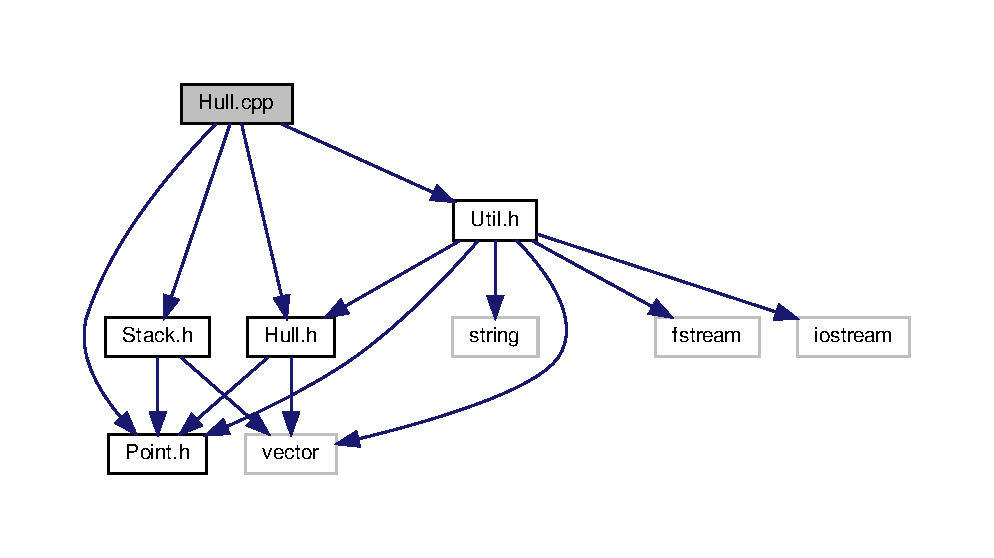
\includegraphics[width=350pt]{Hull_8cpp__incl}
\end{center}
\end{figure}
\subsection*{Functions}
\begin{DoxyCompactItemize}
\item 
int \hyperlink{Hull_8cpp_abe415da8461fb25b5233ff151f55681e}{compare} (const void $\ast$vp1, const void $\ast$vp2)
\begin{DoxyCompactList}\small\item\em This is a comparator function used in Graham Scan to sort the points according to their polar angle wrt to the first point. \end{DoxyCompactList}\end{DoxyCompactItemize}
\subsection*{Variables}
\begin{DoxyCompactItemize}
\item 
\mbox{\Hypertarget{Hull_8cpp_a3986a54502c5144e52a71361fcba7adb}\label{Hull_8cpp_a3986a54502c5144e52a71361fcba7adb}} 
\hyperlink{classUtil}{Util} {\bfseries u}
\item 
\mbox{\Hypertarget{Hull_8cpp_a4fd0aab8d4264b264540df3e0e09dd05}\label{Hull_8cpp_a4fd0aab8d4264b264540df3e0e09dd05}} 
\hyperlink{classStack}{Stack} {\bfseries s}
\end{DoxyCompactItemize}


\subsection{Detailed Description}
This contains all the implementations of the convex hull algorithms. 

\begin{DoxyAuthor}{Author}
your name (\href{mailto:you@domain.com}{\tt you@domain.\+com}) 
\end{DoxyAuthor}
\begin{DoxyVersion}{Version}
0.\+1 
\end{DoxyVersion}
\begin{DoxyDate}{Date}
2019-\/03-\/31
\end{DoxyDate}
\begin{DoxyCopyright}{Copyright}
Copyright (c) 2019 
\end{DoxyCopyright}


\subsection{Function Documentation}
\mbox{\Hypertarget{Hull_8cpp_abe415da8461fb25b5233ff151f55681e}\label{Hull_8cpp_abe415da8461fb25b5233ff151f55681e}} 
\index{Hull.\+cpp@{Hull.\+cpp}!compare@{compare}}
\index{compare@{compare}!Hull.\+cpp@{Hull.\+cpp}}
\subsubsection{\texorpdfstring{compare()}{compare()}}
{\footnotesize\ttfamily int compare (\begin{DoxyParamCaption}\item[{const void $\ast$}]{vp1,  }\item[{const void $\ast$}]{vp2 }\end{DoxyParamCaption})}



This is a comparator function used in Graham Scan to sort the points according to their polar angle wrt to the first point. 


\begin{DoxyParams}{Parameters}
{\em vp1} & const void pointer of type \hyperlink{classPoint}{Point} \\
\hline
{\em vp2} & const void pointer of type \hyperlink{classPoint}{Point} \\
\hline
\end{DoxyParams}
\begin{DoxyReturn}{Returns}
int 
\end{DoxyReturn}

\hypertarget{Hull_8h}{}\section{Hull.\+h File Reference}
\label{Hull_8h}\index{Hull.\+h@{Hull.\+h}}


Header file for \hyperlink{Hull_8cpp}{Hull.\+cpp}.  


{\ttfamily \#include \char`\"{}Point.\+h\char`\"{}}\newline
{\ttfamily \#include $<$vector$>$}\newline
Include dependency graph for Hull.\+h\+:
\nopagebreak
\begin{figure}[H]
\begin{center}
\leavevmode
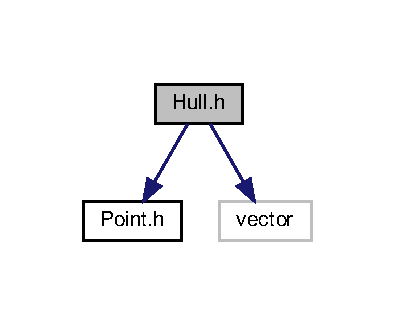
\includegraphics[width=190pt]{Hull_8h__incl}
\end{center}
\end{figure}
This graph shows which files directly or indirectly include this file\+:
\nopagebreak
\begin{figure}[H]
\begin{center}
\leavevmode
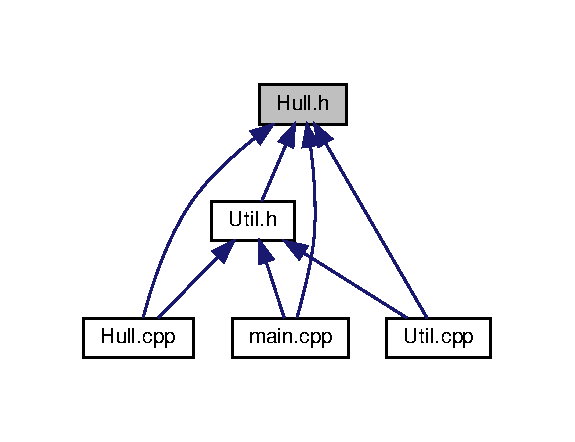
\includegraphics[width=276pt]{Hull_8h__dep__incl}
\end{center}
\end{figure}
\subsection*{Classes}
\begin{DoxyCompactItemize}
\item 
class \hyperlink{classHull}{Hull}
\end{DoxyCompactItemize}
\subsection*{Variables}
\begin{DoxyCompactItemize}
\item 
\mbox{\Hypertarget{Hull_8h_a8593757f85be9886725fdc5bfc5e5e77}\label{Hull_8h_a8593757f85be9886725fdc5bfc5e5e77}} 
\hyperlink{classPoint}{Point} {\bfseries p0}
\end{DoxyCompactItemize}


\subsection{Detailed Description}
Header file for \hyperlink{Hull_8cpp}{Hull.\+cpp}. 

\begin{DoxyAuthor}{Author}
your name (\href{mailto:you@domain.com}{\tt you@domain.\+com}) 
\end{DoxyAuthor}
\begin{DoxyVersion}{Version}
0.\+1 
\end{DoxyVersion}
\begin{DoxyDate}{Date}
2019-\/03-\/31
\end{DoxyDate}
\begin{DoxyCopyright}{Copyright}
Copyright (c) 2019 
\end{DoxyCopyright}

\hypertarget{main_8cpp}{}\section{main.\+cpp File Reference}
\label{main_8cpp}\index{main.\+cpp@{main.\+cpp}}


This is the base file from which all the functions are called.  


{\ttfamily \#include \char`\"{}Point.\+h\char`\"{}}\newline
{\ttfamily \#include \char`\"{}Util.\+h\char`\"{}}\newline
{\ttfamily \#include \char`\"{}Stack.\+h\char`\"{}}\newline
{\ttfamily \#include \char`\"{}Hull.\+h\char`\"{}}\newline
Include dependency graph for main.\+cpp\+:
\nopagebreak
\begin{figure}[H]
\begin{center}
\leavevmode
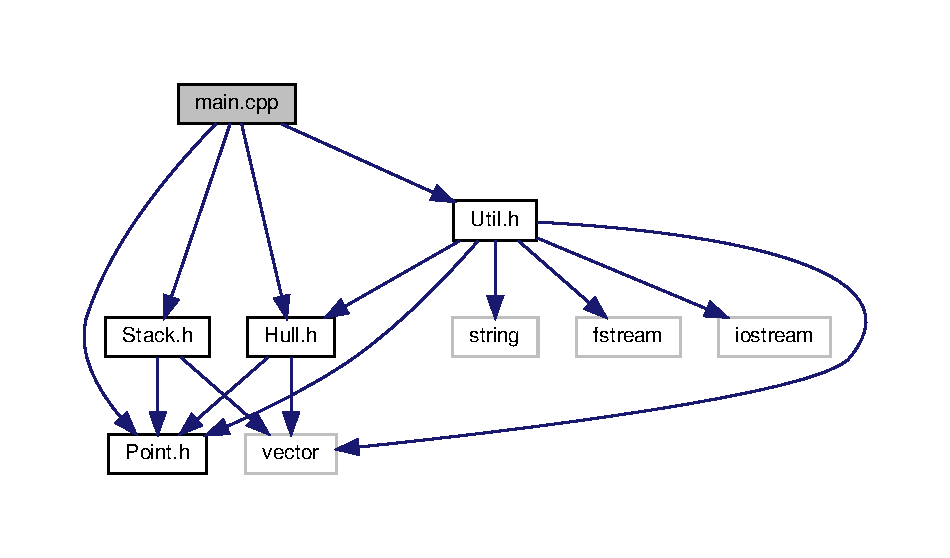
\includegraphics[width=350pt]{main_8cpp__incl}
\end{center}
\end{figure}
\subsection*{Functions}
\begin{DoxyCompactItemize}
\item 
\mbox{\Hypertarget{main_8cpp_a840291bc02cba5474a4cb46a9b9566fe}\label{main_8cpp_a840291bc02cba5474a4cb46a9b9566fe}} 
int {\bfseries main} (void)
\end{DoxyCompactItemize}
\subsection*{Variables}
\begin{DoxyCompactItemize}
\item 
\mbox{\Hypertarget{main_8cpp_ad96b95ae6c2397311bf0a31e11caedf9}\label{main_8cpp_ad96b95ae6c2397311bf0a31e11caedf9}} 
\hyperlink{classHull}{Hull} {\bfseries h}
\item 
\mbox{\Hypertarget{main_8cpp_a8f5a671aa7c0bf36152777d06818d290}\label{main_8cpp_a8f5a671aa7c0bf36152777d06818d290}} 
\hyperlink{classUtil}{Util} {\bfseries f}
\end{DoxyCompactItemize}


\subsection{Detailed Description}
This is the base file from which all the functions are called. 

\begin{DoxyAuthor}{Author}
your name (\href{mailto:you@domain.com}{\tt you@domain.\+com}) 
\end{DoxyAuthor}
\begin{DoxyVersion}{Version}
0.\+1 
\end{DoxyVersion}
\begin{DoxyDate}{Date}
2019-\/03-\/31
\end{DoxyDate}
\begin{DoxyCopyright}{Copyright}
Copyright (c) 2019 
\end{DoxyCopyright}

\hypertarget{Point_8cpp}{}\section{Point.\+cpp File Reference}
\label{Point_8cpp}\index{Point.\+cpp@{Point.\+cpp}}


\hyperlink{classPoint}{Point} Class.  


{\ttfamily \#include $<$iostream$>$}\newline
{\ttfamily \#include \char`\"{}Point.\+h\char`\"{}}\newline
Include dependency graph for Point.\+cpp\+:
\nopagebreak
\begin{figure}[H]
\begin{center}
\leavevmode
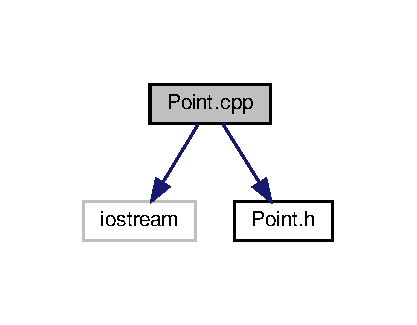
\includegraphics[width=200pt]{Point_8cpp__incl}
\end{center}
\end{figure}


\subsection{Detailed Description}
\hyperlink{classPoint}{Point} Class. 

\begin{DoxyAuthor}{Author}
your name (\href{mailto:you@domain.com}{\tt you@domain.\+com}) 
\end{DoxyAuthor}
\begin{DoxyVersion}{Version}
0.\+1 
\end{DoxyVersion}
\begin{DoxyDate}{Date}
2019-\/03-\/31
\end{DoxyDate}
\begin{DoxyCopyright}{Copyright}
Copyright (c) 2019 
\end{DoxyCopyright}

\hypertarget{Stack_8cpp}{}\section{Stack.\+cpp File Reference}
\label{Stack_8cpp}\index{Stack.\+cpp@{Stack.\+cpp}}


\hyperlink{classStack}{Stack} Class.  


{\ttfamily \#include \char`\"{}Stack.\+h\char`\"{}}\newline
Include dependency graph for Stack.\+cpp\+:
\nopagebreak
\begin{figure}[H]
\begin{center}
\leavevmode
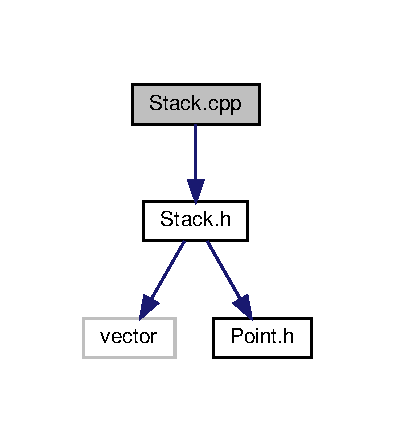
\includegraphics[width=190pt]{Stack_8cpp__incl}
\end{center}
\end{figure}


\subsection{Detailed Description}
\hyperlink{classStack}{Stack} Class. 

\begin{DoxyAuthor}{Author}
your name (\href{mailto:you@domain.com}{\tt you@domain.\+com}) 
\end{DoxyAuthor}
\begin{DoxyVersion}{Version}
0.\+1 
\end{DoxyVersion}
\begin{DoxyDate}{Date}
2019-\/03-\/31
\end{DoxyDate}
\begin{DoxyCopyright}{Copyright}
Copyright (c) 2019 
\end{DoxyCopyright}

\hypertarget{Stack_8h}{}\section{Stack.\+h File Reference}
\label{Stack_8h}\index{Stack.\+h@{Stack.\+h}}


Header file for \hyperlink{classStack}{Stack} Class.  


{\ttfamily \#include $<$vector$>$}\newline
{\ttfamily \#include \char`\"{}Point.\+h\char`\"{}}\newline
Include dependency graph for Stack.\+h\+:
\nopagebreak
\begin{figure}[H]
\begin{center}
\leavevmode
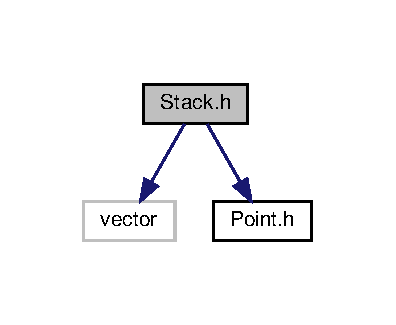
\includegraphics[width=190pt]{Stack_8h__incl}
\end{center}
\end{figure}
This graph shows which files directly or indirectly include this file\+:
\nopagebreak
\begin{figure}[H]
\begin{center}
\leavevmode
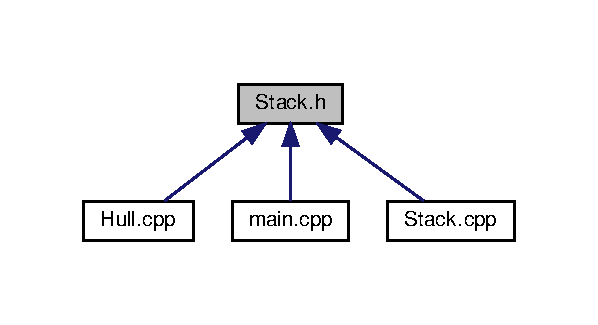
\includegraphics[width=287pt]{Stack_8h__dep__incl}
\end{center}
\end{figure}
\subsection*{Classes}
\begin{DoxyCompactItemize}
\item 
class \hyperlink{classStack}{Stack}
\end{DoxyCompactItemize}


\subsection{Detailed Description}
Header file for \hyperlink{classStack}{Stack} Class. 

\begin{DoxyAuthor}{Author}
your name (\href{mailto:you@domain.com}{\tt you@domain.\+com}) 
\end{DoxyAuthor}
\begin{DoxyVersion}{Version}
0.\+1 
\end{DoxyVersion}
\begin{DoxyDate}{Date}
2019-\/03-\/31
\end{DoxyDate}
\begin{DoxyCopyright}{Copyright}
Copyright (c) 2019 
\end{DoxyCopyright}

\hypertarget{Util_8cpp}{}\section{Util.\+cpp File Reference}
\label{Util_8cpp}\index{Util.\+cpp@{Util.\+cpp}}


\hyperlink{classUtil}{Util} Class which contains all the helper functions used in the convex hull algorithms.  


{\ttfamily \#include \char`\"{}Util.\+h\char`\"{}}\newline
{\ttfamily \#include \char`\"{}Hull.\+h\char`\"{}}\newline
{\ttfamily \#include $<$math.\+h$>$}\newline
Include dependency graph for Util.\+cpp\+:
\nopagebreak
\begin{figure}[H]
\begin{center}
\leavevmode
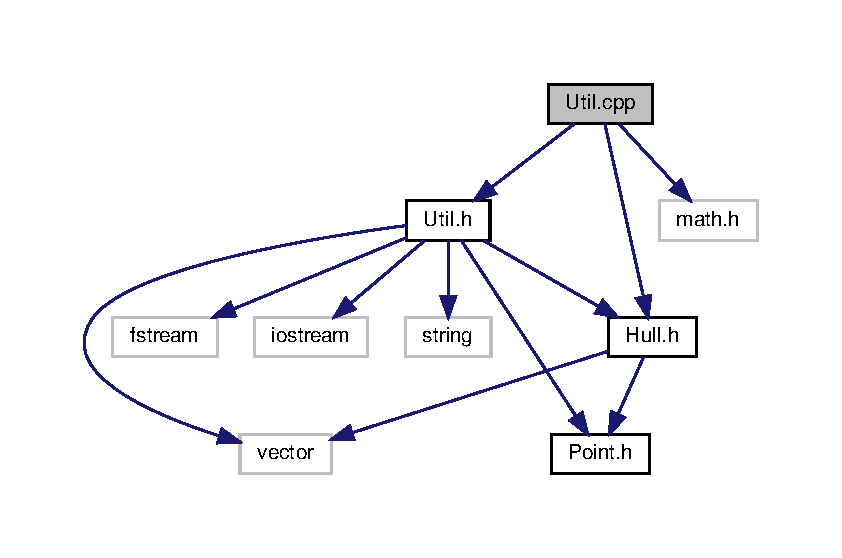
\includegraphics[width=350pt]{Util_8cpp__incl}
\end{center}
\end{figure}
\subsection*{Variables}
\begin{DoxyCompactItemize}
\item 
\mbox{\Hypertarget{Util_8cpp_a8593757f85be9886725fdc5bfc5e5e77}\label{Util_8cpp_a8593757f85be9886725fdc5bfc5e5e77}} 
\hyperlink{classPoint}{Point} {\bfseries p0}
\end{DoxyCompactItemize}


\subsection{Detailed Description}
\hyperlink{classUtil}{Util} Class which contains all the helper functions used in the convex hull algorithms. 

\begin{DoxyAuthor}{Author}
your name (\href{mailto:you@domain.com}{\tt you@domain.\+com}) 
\end{DoxyAuthor}
\begin{DoxyVersion}{Version}
0.\+1 
\end{DoxyVersion}
\begin{DoxyDate}{Date}
2019-\/03-\/31
\end{DoxyDate}
\begin{DoxyCopyright}{Copyright}
Copyright (c) 2019 
\end{DoxyCopyright}

\hypertarget{Util_8h}{}\section{Util.\+h File Reference}
\label{Util_8h}\index{Util.\+h@{Util.\+h}}


Header file for \hyperlink{classUtil}{Util} Class.  


{\ttfamily \#include $<$fstream$>$}\newline
{\ttfamily \#include $<$iostream$>$}\newline
{\ttfamily \#include $<$string$>$}\newline
{\ttfamily \#include $<$vector$>$}\newline
{\ttfamily \#include \char`\"{}Point.\+h\char`\"{}}\newline
{\ttfamily \#include \char`\"{}Hull.\+h\char`\"{}}\newline
Include dependency graph for Util.\+h\+:
\nopagebreak
\begin{figure}[H]
\begin{center}
\leavevmode
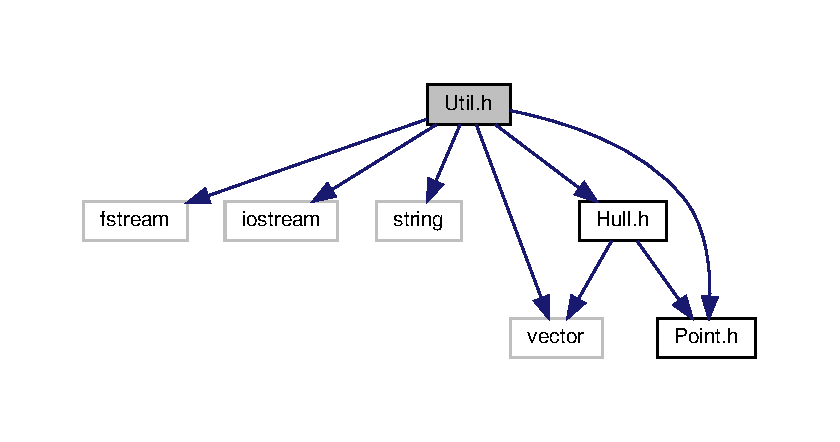
\includegraphics[width=350pt]{Util_8h__incl}
\end{center}
\end{figure}
This graph shows which files directly or indirectly include this file\+:
\nopagebreak
\begin{figure}[H]
\begin{center}
\leavevmode
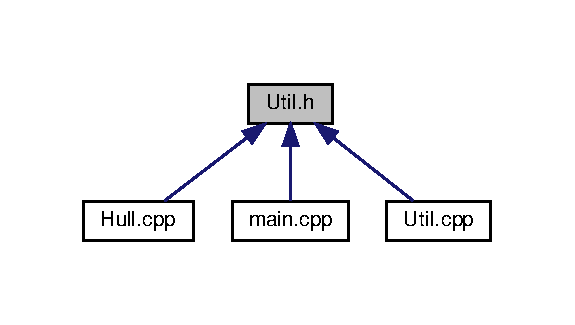
\includegraphics[width=276pt]{Util_8h__dep__incl}
\end{center}
\end{figure}
\subsection*{Classes}
\begin{DoxyCompactItemize}
\item 
class \hyperlink{classUtil}{Util}
\end{DoxyCompactItemize}


\subsection{Detailed Description}
Header file for \hyperlink{classUtil}{Util} Class. 

\begin{DoxyAuthor}{Author}
your name (\href{mailto:you@domain.com}{\tt you@domain.\+com}) 
\end{DoxyAuthor}
\begin{DoxyVersion}{Version}
0.\+1 
\end{DoxyVersion}
\begin{DoxyDate}{Date}
2019-\/03-\/31
\end{DoxyDate}
\begin{DoxyCopyright}{Copyright}
Copyright (c) 2019 
\end{DoxyCopyright}

%--- End generated contents ---

% Index
\backmatter
\newpage
\phantomsection
\clearemptydoublepage
\addcontentsline{toc}{chapter}{Index}
\printindex

\end{document}
